	\documentclass[10pt,conference]{IEEEtran}

\usepackage{cite}
\ifCLASSINFOpdf
   \usepackage[pdftex]{graphicx}
   \graphicspath{{figs/}}
   \DeclareGraphicsExtensions{.pdf,.jpeg,.png}
\else
   \usepackage[dvips]{graphicx}
   \graphicspath{{../figs/}}
   \DeclareGraphicsExtensions{.eps}
\fi

\usepackage[cmex10]{amsmath}
\interdisplaylinepenalty=2500
\usepackage{amsthm}
\newtheorem{definition}{Definition}
\usepackage{algorithmic}
\usepackage{array}
\usepackage{subcaption}
\usepackage{url}
\usepackage[T1]{fontenc}
\usepackage[utf8]{inputenc}
\usepackage[brazilian]{babel}

% corrija hifenação aqui
\hyphenation{op-tical net-works semi-conduc-tor}

\usepackage{hyperref}
\usepackage{listings}
\usepackage{xcolor}

\definecolor{codegreen}{rgb}{0,0.6,0}
\definecolor{codegray}{rgb}{0.5,0.5,0.5}
\definecolor{codepurple}{rgb}{0.58,0,0.82}
\definecolor{backcolour}{rgb}{0.95,0.95,0.92}

\lstdefinestyle{mystyle}{
    backgroundcolor=\color{backcolour},   
    commentstyle=\color{codegreen},
    keywordstyle=\color{magenta},
    numberstyle=\tiny\color{codegray},
    stringstyle=\color{codepurple},
    basicstyle=\ttfamily\footnotesize,
    breakatwhitespace=false,         
    breaklines=true,                 
    captionpos=b,                    
    keepspaces=true,                 
    numbers=left,                    
    numbersep=5pt,                  
    showspaces=false,                
    showstringspaces=false,
    showtabs=false,                  
    tabsize=2
}

\lstset{style=mystyle}

\begin{document}
\title{Relatório - Sistemas Distribuídos \\
    \large{Difusão Atômica utilizando Mecanismo de Ordenação Total Baseado em Privilégio e Algoritmo de Exclusão Mútua Distribuída Baseado em Anel}}

\newif\iffinal
\finalfalse
\finaltrue
\newcommand{\jemsid}{99999}

\iffinal
\author{\IEEEauthorblockN{Christiane Fernandes Peressutti}
\IEEEauthorblockA{Engenharia de Computação \\
Universidade Federal de Santa Catarina - UFSC\\
Email: christiane.peressutti@grad.ufsc.br}
%\and
%\IEEEauthorblockN{Aluno 2}
%\IEEEauthorblockA{Engenharia da Computação\\
%INSPER\\
%Email: aluno2@insper.edu.br}
}

\else
  \author{Sibgrapi paper ID: \jemsid \\ }
\fi


\maketitle

\begin{abstract}
Serão tratadas duas implementações relacionadas a sistemas distribuídos, sendo estas de difusão atômica com mecanismo de ordenação total baseado em privilégio e algoritmo de exclusão mútua distribuído baseado em anel, sendo ambas representadas a seguir em códigos com saídas intuitivas quanto a seu funcionamento.
%Um resumo de 100-200 palavras do seu trabalho. Deve conter, brevemente, motivação, problema estudado, solução proposta/implementada e resultados obtidos.
\end{abstract}
\IEEEpeerreviewmaketitle

\section{Introdução}
Em sistemas distribuídos, diversos conceitos são abordados quanto a processos, comunicação entre processos distribuídos, concorrência e sincronização, tolerância a faltas, segurança e seus estudos de caso. 

Serão expostas implementações e conceitos quanto a difusão atômica utilizando o mecanismo de ordenação total baseado em privilégio e ao algoritmo de exclusão mútua distribuído baseado em anel.

Visto que suas representações poderão ser de forma gráfica ou escrita, a linguagem de programação escolhida foi Python.

%Sua introdução deve responder às seguintes perguntas:

%\begin{enumerate}
%\item Qual a motivação do trabalho? (Por que o problema estudado é útil?)
%\item Qual é o problema estudado?
%\item Quais dificuldades existem?
%\item Qual a solução proposta e como ela se relaciona com as dificuldades existentes?
%\item Como a solução será avaliada? (Quais testes serão feitos para mostrar que o projeto funciona?)
%\end{enumerate}

\section{Difusão Atômica com Mecanismo de Ordenação Total Baseada em Privilégio}
\subsection{Conceito}
O funcionamento do mecanismo de ordenação total baseada em privilégio divide-se em duas partes prinicpais, sendo os remetentes (emissores) e os destinatários (receptores). 

Funciona da seguinte forma: os emissores formam um anel virtual no qual circula um token, cujo emissor que estiver de posse deste tem o privilégio de difundir suas mensagens \cite{compdistlau}, como ilustrado abaixo. As mensagens enviadas tem mesmo conteúdo e ordem de chegada.

\begin{figure} [h]
    \centering
    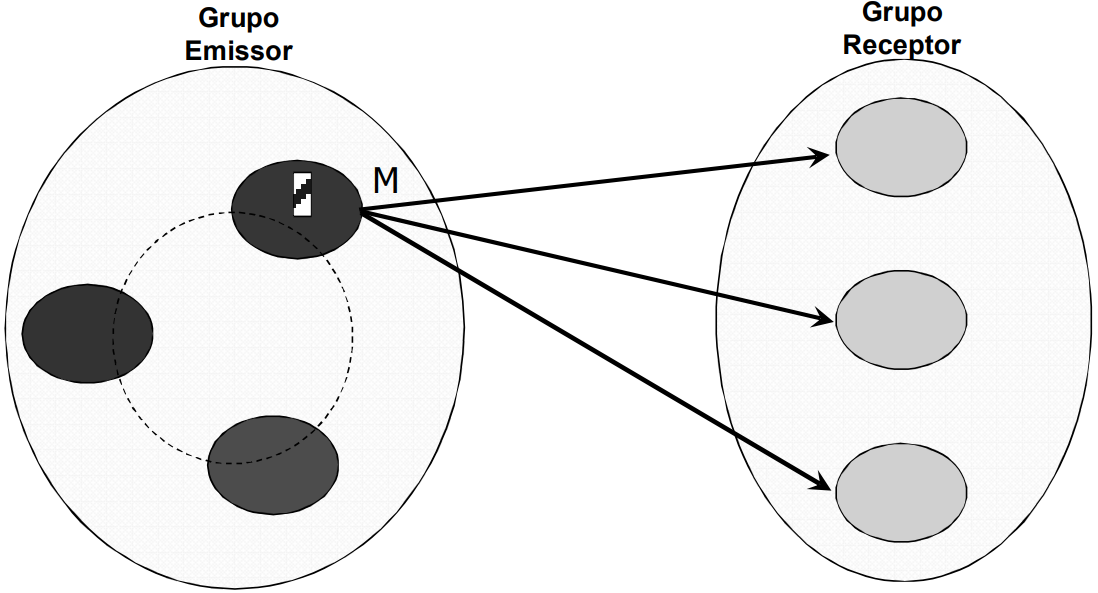
\includegraphics[width=8.5cm]{images/baseadoempriv.png}
    \caption{Funcionamento do mecanismo de ordenação total baseado em privilégio} 
    \label{fig:enter-label}
\end{figure}

Por parte dos emissores, o algoritmo é inicializado com um conjunto vazio. Para o primeiro processo inicializa-se o token com 1 e executa-se a primitiva que enviará o token para o primeiro processo. Em seguida, executa-se a difusão de ordem total sobre a mensagem, que é unida ao conjunto. Ao receber o novo token, cada mensagem dentro do conjunto executa a primitiva de envio com o valor atual do token, que irá rotacionar, para os receptores. O token é enviado para o próximo processo após ser feito um cálculo modular que itera pelos processos participantes de forma anelar, que ao receber executa novamente o algoritmo \cite{defago2000totally}. 

Já o algoritmo do receptor inicializa os conjunto de dados de próxima entrega com todos os valores igual à 1 e fim como vazio. Em seguida, começa a processar continuamente o recebimento de mensagens, cada uma com seu número de sequência. Logo após, implementa a união de novas mensagens no conjunto de pendências em laço repetitivo, onde se verifica a existência de uma mensagem com número de sequência pertencente ao conjunto de pendências. Caso sim, o número de sequência receberá o valor da próxima entrega. Em sequência, executa a primitiva de entrega \cite{defago2000totally}.    

Esta técnica pode apresentar alguns problemas, sendo a perda do token caso haja falha no processo que o esteja usando \cite{compdistlau}.

\subsection{Implementação}
Dada a descrição do algoritmo anteriormente, abaixo encontra-se o código implementado para demonstração do funcionamento. O número de processos do remetente pode ser alterado na chamada da linha 7 \verb|numproc = 3|.

\begin{lstlisting}[language=Python, caption=Código main]
    from emissor import process
    from receptor import process_pi
    from comunica import send
    
    def main():
        i=0
        numproc = 3
        
        if i <= numproc:
                r = process(numproc)
                e = process_pi()

    if __name__ == '__main__':
        main()
\end{lstlisting}

\begin{lstlisting}[language=Python, caption= Código do Emissor]
    from receptor import receive
    from comunica import send
    
    def TO_broadcast(m):
        global tosendsi
        tosendsi.append(m)
    
    def process(si):
        global token, seqnum
        global tosendsi
        token = 'teste'
        seqnum = 0
        destino = "127.0.0.1"
        tosendsi = []
        s1 = 1
    
        if si == s1:
            seqnum +=1
            send(token, s1, destino)
            print('enviado')
            si += 1
            
        boole = True
        while boole:
            receive(token, seqnum)
            for m_prime in tosendsi:
                
                send(m_prime, token.seqnum, destino)
                print('enviado')
                #token(seqnum := token.seqnum+1) 
                seqnum +=1 
                si += 1
                  
            tosendsi = []
       
            send(token, (si+1), destino)
            print('enviado')
            
            parar = 1
            if parar >= 1:
                #time.sleep(0.5)
                boole = False
\end{lstlisting}

\begin{lstlisting}[language=Python, caption=Código do Receptor]
    nextdeliverpi = 0
    pendingpi = []
    
    def receive(m, seqnum):
        pendingpi.append((m, seqnum))
        print("todas as mensagens recebidas: ", pendingpi)
    
    def deliver(m):
        print("mensagem recebida: ", m)
    
    def process_pi():
        global nextdeliverpi
        boole = True
        while boole:
            for i, (m, seqnum) in enumerate(pendingpi):
                if seqnum == nextdeliverpi:
                    deliver(m)
                    nextdeliverpi += 1
                    pendingpi.pop(i)
                    break
\end{lstlisting}

\begin{lstlisting}[language=Python, caption=Código de Envio de Mensagem]
    import socket

    def send(message, seqnum, destination):
        # Cria um socket UDP
        with socket.socket(socket.AF_INET, socket.SOCK_DGRAM) as s:
            m = message.encode()
    
            # Envia a mensagem para o destino
            s.sendto(m, (destination, 5000))    
\end{lstlisting}

\section{Algoritmo de Exclusão Mútua Distribuído Baseado em Anel}
\subsection{Conceito}
O algoritmo de exclusão mútua distribuído baseado em anel (token ring) é formado por um grupo não ordenado de processos. É embasado na topologia lógica de anel construído em software. Nesse anel, cada processo, antes encontrados em uma rede de barramento, será designado a uma posição, que pode ser alocado em ordem numérica de endereços de rede ou outro meio \cite{compdistaline}. 

\begin{figure}[h]
    \centering    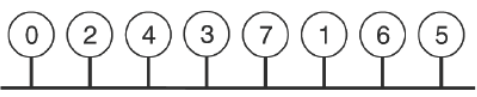
\includegraphics[width=8.5cm]{images/exclusaomutuaanel.png}
    \caption{Processos na rede desordenados}
    \label{fig:enter-label}
\end{figure}
\begin{figure}[h]
    \centering    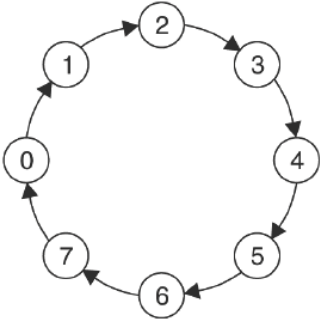
\includegraphics[width=8.5cm]{images/exclusaomutuaanel2.png}
    \caption{Anel lógico inicializado}
    \label{fig:enter-label}
\end{figure}

Quando o anel é inicializado, o processo 0 recebe uma ficha (token), que circula ao redor do anel. Quando um processo adquire o token de seu vizinho, ele verifica se está tentando entrar em uma região crítica. Nesse caso, o processo entra na região, faz todo o trabalho necessário e sai da região. Depois de sair, ele passa o token para o próximo processo no anel. Não é permitido entrar novamente na região crítica utilizando o mesmo token. Se um processo recebe o token de seu vizinho e não está interessado em entrar em uma região crítica, ele apenas passa o token para o próximo processo. \cite{tanenbaum}

Apenas um processo pode obter o recurso por vez, evitando assim inanição. Todavia, se o token for perdido, precisará ser regenerado, considerando que a quantidade de tempo entre aparições sucessivas do token na rede é ilimitado. Ademais, se um processo cair, poderá ser removido do grupo, passando o token para o próximo. Para isso, todos precisam manter a configuração corrente do anel. \cite{tanenbaum}

\subsection{Implementação}
Como no tópico visto precedentemente, abaixo encontra-se o código implementado para demonstração do funcionamento. O número de nodos pode ser alterado na chamada da linha 41 \verb|num_nodes = 7|. 

\begin{lstlisting}[language=Python, caption=Código de implementação do Algoritmo de Exclusão Mútua Distribuído Baseado em Anel]
    import threading
    
    class Token: #token que e passado entre os nos do anel
        def __init__(self, value):
            self.value = value
    
    class Node(threading.Thread): #representa cada no do anel. Cada no e executado em uma thread separada e possui um identificador, um token e uma referencia para o proximo no no anel
        def __init__(self, id):
            super().__init__()
            self.id = id
            self.token = None
            self.next_node = None
    
        def run(self): #verifica se possui o token. Se possuir, entra na secao critica e imprime uma mensagem. Caso contrario, passa o token para o proximo no
            while True:
                if self.token is not None:
                    if self.token.value == self.id:
                        print(f"Nodo {self.id} na secao critica com {self.token}\n")
                        self.token = None
                        print(f"Nodo {self.id} agora com {self.token}\n")
                    else:
                        self.pass_token()
                #else:
                #    self.receive_token(self.next_node.token)
    
        def pass_token(self): #passa o token para o proximo no
            self.next_node.receive_token(self.token)
            print(f"Seguiu para o proximo {self.next_node.id} com token: \n", self.token)
            self.token = None
    
        def receive_token(self, token): #recebe o token de um no anterior
            if token is not None:
                self.token = token
                print("Recebeu token: \n", token)
    
        def set_next_node(self, next_node): #seta para o proximo nodo
            self.next_node = next_node
            print("Proximo: \n", next_node)
    
    def main(): #sao criados os nos e configuradas as referencias para o proximo no. Em seguida, cada no e iniciado em uma thread separada
        num_nodes = 7
        nodes = []
    
        for i in range(num_nodes):
            #next_node = nodes[i].set_next_node(nodes[(i + 1) % num_nodes])
            node = Node(i)
            nodes.append(node)
    
        for i in range(num_nodes):
                nodes[i].set_next_node(nodes[(i + 1) % num_nodes])
    
    
        for node in nodes:
            node.token = Token(node.id) # define o token inicial para cada no
            threading.Thread(target=node.run).start()
    
    if __name__ == "__main__":
        main()
\end{lstlisting}

\section*{Execução dos Códigos}
Para executar os códigos apresentados será preciso instalar uma IDE da preferência do leitor, com indicação para \href{https://code.visualstudio.com/download}{VSCode}, \href{https://docs.spyder-ide.org/3/installation.html}{Spyder} ou IDLE (este instalado junto ao Python). 

Fazer a instalação do \href{https://www.python.org/downloads/}{Python} de versão posterior a 3.6. Ao abrir o executável de instalação selecionar a opção para incluir ao PATH.

Abrir a pasta contendo o código na IDE e selecionar a opção de executar, executar e depurar ou utilizar o comando: \verb|python main.py|

Caso escolha pelo VSCode, antes do passo anterior, com o comando \verb|crtl + shift + P| selecionar o interpretador correspondente a versão do Python. 

%\section{Método/Solução proposto(a)}

%Descreva aqui com detalhes tudo o que foi realizado no projeto. Lembre-se que é mais importante descrever a ideia que foi usada para criar o código do que o código em si. A descrição de como o projeto está organizado fica no repositório do código. 

%\section{Resultados / Avaliação dos resultados}

%Descreva nesta seção quais são os resultados esperados de maneira mais detalhada e o que vocês farão para verificar se os resultados foram cumpridos. É importante pensar em como medir o sucesso do projeto (qual porcentagem de vezes o robô realizou a tarefa corretamente? se é projeto de localização, qual o erro entre a posição real e a estimada? etc ) e analisar com alguma profundidade os erros cometidos (se errou, qual parte do método proposto falhou?)

%Exemplo:

%Para testar a eficácia do método proposto na tarefa XYZ realizaremos os seguintes experimentos:

%\begin{enumerate}
%\item executar tarefa no contexto ABC;
%\item testar robustez à situação A;
%\item verificar se o método funciona na situação B.
%\end{enumerate}

%No contexto ABC o método proposto resolveu a tarefa corretamente em 4 de 5 execuções. Na execução sem sucesso a parte ABC do método não funcionou.

\section{Considerações Finais}
Neste relatório foram apresentados conceitos e funcionamento dos algoritmos, bem como suas implementações Todo código está disponível no \href{https://github.com/christalfepe/Sistemas-Distribu-dos.git}{repositório}. Podem ocorrer alguns problemas na execução do código baseado em privilégio que até o fim deste relatório não foram solucionados, de forma que precisarão ser resolvidos adiante. Além disto, a implementação de saída gráfica não fora possível por conta de problemas de renderização.

%\section{Conclusão}
%Relembre os pontos descritos na introdução e avalie se eles foram cumpridos. Relembre os pontos positivos e negativos do método usado no projeto.

%\section*{Recursos para aprender \LaTeX}

%Os dois sites abaixo são excelentes fontes para aprender \LaTeX e devem ser consultados antes de perguntar para os professores ;)

%\begin{itemize}
%\item https://en.wikibooks.org/wiki/LaTeX
%\item https://tex.stackexchange.com
%\end{itemize}

\bibliographystyle{IEEEtran}
\bibliography{example}
\end{document}


